\section{Einleitung}
	\subsection{Forschungsfrage und Zielsetzung}	 
	Seit dem 30. November 2022 ist der Chatbot ChatGPT veröffentlicht und frei nutzbar. 
	Nach weniger als zwei Monaten konnte ChatGPT bereits 100 Millionen Nutzer verzeichnen \cite[S. 15]{spitzer23}.
	Aufgrund des großen Erfolgs begannen nach kurzer Zeit auch andere Unternehmen wie Google eigene 
	Chatbots zu trainieren. Mittlerweile gibt es immer umfangreichere und leistungsfähigere KI\footnote{Künstliche Intelligenz} 
	und ihre Entwicklung schreitet rasant voran.	
	
	Diese Technologie hat auch einen immer größeren Einfluss auf unsere moderne Gesellschaft. 
	Chatbots gehören für viele Menschen bereits zum Alltag und helfen in der Schule, im Studium und im Beruf, 
	beispielsweise beim Verfassen längerer Texte \cite[S. 175, S. 185]{shaji23}.
	Auf der anderen Seite gibt es aber auch Chatbots, die keinen praktischen Nutzen haben und dazu gedacht sind,
	sich die Zeit zu vertreiben, indem man z.B. emotionale Gespräche mit ihnen führt. Diese Art von Chatbots spielt 
	vor allem aus sozialer Sicht eine zunehmende Rolle. 
	
	Aus diesen Gründen ist es wichtig, diese Technologie richtig einordnen zu können. Allerdings wissen nur wenige
	wie Chatbots funktionieren, was dazu führt, dass ihre Fähigkeiten oft falsch eingeschätzt werden. 
	Daher soll in dieser Arbeit der Frage nachgegangen werden, welches Bild die Öffentlichkeit von 
	Chatbots hat bzw. was an diesem Bild problematisch ist. 
	
	Diese Arbeit verfolgt das Ziel aufzuzeigen, wie es bei der Berichterstattung über KI zu Problemen
	kommen kann. Außerdem wird die soziale Nutzung von KI-Chatbots diskutiert. Daraus soll erschlossen 
	werden, wie die Öffentlichkeit über KI-Dialogsysteme denkt und warum dadurch ein falscher Eindruck von 
	Chatbots bzw. KI entstehen kann. Aufgrund dessen wird näher auf die Funktionsweise dieser Programme 
	eingegangen. Nach dem Lesen der Arbeit soll man ein grundlegendes Verständnis von Chatbots haben und 
	mit Informationen diesbezüglich aufgeschlossener umgehen können. 

	\clearpage
	\subsection{Methodik und Aufbau} 
	Im ersten Teil der Arbeit werden verschiedene Beispiele behandelt, die zeigen, dass leicht ein falscher 
	Eindruck von KI, insbesondere Chatbots, entstehen kann. Zunächst wird auf die soziale Bedeutung von
	KI-Chatbots eingegangen, und die damit verbundenen Konsequenzen und Auswirkungen näher erläutert. Anschließend
	wird anhand populärwissenschaftlicher Artikel gezeigt, dass die Funktionsweise von KI häufig missverständlich 
	oder ungenau dargestellt wird, was in solchen Quellen leicht zu Missverständnissen führen kann.
	Darauf folgt eine grundlegende Betrachtung des Themas Chatbots und IQ-Tests. Zunächst wird erläutert, welche
	Bedeutung IQ-Tests im Zusammenhang mit Chatbots haben. Des Weiteren wird gezeigt, was man bei der Auswertung von 
	Ergebnissen, die Chatbots in IQ-Tests erzielen, beachten muss.

	Das darauffolgende Kapitel behandelt die Funktionsweise von Chatbots. Zunächst werden einige wichtige Begriffe geklärt. 
	Es folgt eine Einführung in LLM und GPT. Die grundlegende Funktionsweise von KI-Chatbots wird dabei auf leicht  
	verständliche Weise vermittelt. Mit diesen neuen Erkenntnissen wird anschließend das Thema AGI behandelt. Anhand von ausgewählten
	Beispielen wird verdeutlicht, warum wir derzeit noch keine Allgemeine Künstliche Intelligenz verwenden. Dieses Thema ist hier
	besonders passend, da im ersten Teil der Arbeit bereits gezeigt wurde, dass moderne KI häufig falsch dargestellt wird und die 
	Unterscheidung zwischen AGI und ANI (die KI, die wir verwenden) oft schwerfällt.

	Im abschließenden Teil der Arbeit sollen Missverständnisse und Problematiken aus dem ersten Teil geklärt werden. Zunächst wird 
	darauf hingewiesen, dass KI derzeit keine menschlichen Gefühle oder Emotionen besitzt. Anschließend werden Missverständnisse aus
	den zuvor behandelten Artikeln aufgeklärt. Zuletzt wird die Problematik bei der Auswertung von IQ-Tests,
	die von Chatbots bearbeitet wurden, diskutiert. 	
	
	
\clearpage
\section{Die öffentliche Wahrnehmung von Chatbots}\label{s1}
	\subsection{Chatbots mit Gefühlen?}\label{s1ss1}
	Eine kurze Erklärung vorab: Die meisten kennen bekannte Chatbots wie ChatGPT, die dazu
	entwickelt wurden, uns bei diversen Aufgaben zu unterstützen. Im Gegensatz dazu steht Character.AI, 
	eines der Unternehmen, die \glqq{}persönliche\grqq{} AEI\footnote{Artificial Emotional Intelligence} 
	anbieteten \cite{cAI24}. Das bedeutet, dass die KI darauf ausgelegt ist, soziale Gespräche zu führen.
	Man kann zwischen verschiedenen Chatbots, die größtenteils fiktive Charaktere repräsentieren, wählen. Sie
	sind darauf ausgelegt möglichst emotional und menschlich zu reagieren und oft stehen dabei sehr 
	persönliche Themen im Vordergrund, z. B. Einsamkeit, Freundschaft, Empathie oder sogar Liebesbeziehungen. 
	
	Das dabei eine emotionale Bindung zu Chatbots entsteht, ist durchaus möglich und dafür reicht ein 
	Chatbot aus, der nur begrenzte soziale Fähigkeiten besitzt \cite{chen24}. KI ist für viele Menschen also 
	nicht nur eine praktische Anwendung, die im Alltag hilfreich ist, sondern hat für einige Personen auch
	emotionalen Mehrwert. Ob und warum dies kritisch betrachtet werden muss, wird in \ref{s3ss1} diskutiert.  

	Character.AI ist nur eines von mehreren Unternehmen, die persönliche AEI anbieten und das mit Erfolg. 
	Seit September 2022 ist Character.AI frei verfügbar und hat zum jetzigen Zeitpunkt August 2024 bereits
	über 10 Millionen Downloads bei Google Play. Aufgrund der schnellen Weiterentwicklung von KI und des 
	global stärker werdenden Gefühls von Einsamkeit ist demnach zu erwarten, dass die soziale Bedeutung 
	von Chatbots zunehmen wird \cite{chen24}. 
	
	
	\clearpage		
	\subsection{Mediale Berichterstattung}\label{s1ss2}
	Die Medien spielen bei der Berichterstattung über KI eine entscheidende Rolle. Sie tragen nicht nur dazu
	bei, die Öffentlichkeit über aktuelle Entwicklungen und Innovationen zu informieren, sondern sind auch 
	verantwortlich dafür, komplexe technische Zusammenhänge verständlich zu vermitteln. Doch genau hier kann
	es auch zu Problemen kommen, wodurch eine falsche Auffassung von aktuellen Chatbots entsteht.

	Ein Beispiel hierfür ist das Demonstrationsvideo von Google zu ihrem Chatbot Gemini \cite{gminiDemo2023}. 
	Das Video zeigt eine Person, die mit dem Chatbot Gemini live interagiert und ihm Fragen stellt. Dabei
	zeichnet die Person beispielsweise ein Bild von einer Ente und stellt dem Chatbot immer wieder Fragen dazu.
	Später im Video deutet die Person durch Handbewegungen an, dass sie mit dem Chatbot das Spiel \glqq{}Schere
	Stein Papier\grqq{} spielen will. Der Chatbot antwortet, dass er die Herausforderung annimmt. Das Video
	betont dadurch vor allem die Interaktivität zwischen Gemini und der anwesenden Person. Außerdem zeigt das
	Video einen autonomen Chatbot, der aus einem bestimmten Kontext erschließt welche Antwort gefragt ist. 

	In vielen Artikeln zu Chatbots wird deren Funktionsweise und Training erklärt. Maria Gramsch erklärt in 
	ihrem Artikel wie ChatGPT funktioniert. Sie fasst sich hierbei kurz und erklärt unter anderem
	auch das Training von Chatbots. In dem Artikel ist mehrmals zu lesen, dass das Training von ChatGPT stets
	unvollendet ist und dass der Chatbot aus Konversationen mit den Nutzern immer weiter dazu lernt \cite{gramsch23}. 
	Dadurch wird der Eindruck vermittelt, dass ChatGPT wie ein Mensch aus seinen Erfahrungen lernt.

	Was genau an den genannten Beispielen zur Berichterstattung falsch ist, wird in \ref{s3ss2} verdeutlicht. 
	Es steht aktuell eine Vielzahl an Möglichkeiten zur Verfügung, um sich über KI und Chatbots zu informieren. 
	Dadurch kann es schwierig werden eine korrekte Informationsquelle zu wählen, die gut verständlich ist.   	 	 
	
	\clearpage
	\subsection{Chatbots und IQ-Tests}\label{s1ss3}
	Mit der steigenden Zahl an KI Modellen, wird KI-Benchmarking\footnote{Vergleich von KI-Systemen} immer wichtiger. 
	Außerdem stellt sich die Frage, wie intelligent ein Chatbot verglichen mit einem Menschen ist. IQ-Tests 
	bieten eine Möglichkeit das zu tun, sie sind dazu entworfen Intelligenz so gut wie möglich zu messen und das 
	funktioniert auch bei KI. Jedoch ist es wichtig die Ergebnisse, welche KI in IQ-Tests erzielt, kritisch zu
	sehen und richtig zu deuten.

	Eka Roivainen schreibt in seinem Artikel, wie er mit dem damals neu veröffentlichten ChatGPT-4 einen IQ-Test
	durchgeführt hat \cite{roivainen23}. Er schildert zu Beginn des Artikels, dass er sich dafür interessiere, wie
	schlau ChatGPT im Vergleich zu menschlichen Standards ist. Im verbalen Teil des verwendeten WAIS-III Tests
	erklärt er, der Chatbot hat einen Wert von 155 erzielt und ist damit besser als \mbox{99,9 \%} der menschliche Teilnehmer.
	Der Artikel wurde in anderen Artikeln zitiert, wie beispielsweise von Sandra Blütermann in ihrem Artikel
	\cite{blutermann23}. In einem Interview von Sky News Australia sagt Mo Gawdat, ein ehemaliger Chief Business
	Officer von Google, ebenfalls, dass ChatGPT einen IQ von 155 habe und damit fast so intelligent wie Albert Einstein
	sei \cite{gawdat23}.

	Betrachtet man das Ergebnis, was Roivainen mit ChatGPT-4 in ihrem IQ-Test erzielt hat, könnte man meinen,
	dass KI dem Menschen bereits überlegen ist. Mo Gawdat sagt das sogar schon fast wörtlich in seinem Interview:
	\glqq{}Der IQ von ChatGPT-4 wird auf 155 geschätzt, das ist viel schlauer als der durchschnittliche Mensch\grqq{} 
	\cite{gawdat23}. In \ref{s3ss3} werden die Ergebnisse, von ChatGPT-4 im WAIS-III Test genauer betrachtet.
	Darüber hinaus wird die Aussage von Mo Gawdat über die Intelligenz von ChatGPT-4, diskutiert und widerlegt. 	

\clearpage	
\section{Die Funktionsweise von KI-Dialogsystemen}
	\subsection{Begriffe und Grundlagen}\label{s2ss1}
	Um das nächste Kapitel verstehen zu können, müssen zunächst einige wichtige Begriffe und Sachverhalte erklärt 
	werden. Natürlich kann im Rahmen dieser Arbeit keine komplette Erklärung rund um LLM und GPT bis ins Detail
	gewährleistet werden, darum beziehe ich mich auf das Nötigste, damit man die folgenden Teile der Arbeit gut verstehen
	kann: 
	
	\begin{itemize}
		\item \textbf{Neuronale Netze}: Man kann ein neuronales Netz als eine mathematische Funktion sehen,
		die eine Anzahl $n$ an Werten annimmt und eine Anzahl $m$ an Werten ausgibt. Diese Werte kann man auch als Eingabe-
		und Ausgabevektor sehen: 		
		
		\begin{equation*}	
			f(\vec{v}) = \vec{w}\textnormal{,\qquad wobei } \vec{v} \in \mathbb{R}^n \textnormal{ und } \vec{w} \in \mathbb{R}^m
		\end{equation*}  
		\vspace{0.0cm}
		
		Die Funktion $f$ hat zahlreiche Parameter (175 Milliarden bei GPT-3 \cite[S. 8]{openAI2020}), die man genau so 
		anpassen will, dass aus unterschiedlichen Eingabevektoren die gewünschten Ausgabevektoren werden und genau hier kommt 
		das Training ins Spiel. Durch Training ist es möglich, die zahlreichen Parameter des Netzwerks so anzupassen, dass 
		sich die Werte der Ausgabevektoren möglichst gut an die gewünschten Werte annähern \cite[S. 127f]{nielsen2015}. Bei
		der Verwendung eines neuronalen Netzwerks findet keine Veränderung der Parameter statt.   

		\item \textbf{Schicht eines Neuronalen Netzwerks}: Ein neuronales Netzwerk ist in mehrere Schichten unterteilt, die verschiedene
		Bearbeitungsschritte darstellen. Die Eingabevektoren durchlaufen jede Schicht und werden dabei schrittweise in die Ausgabevektoren
		umgerechnet \cite[S. 4]{nielsen2015}. 
		
		\item \textbf{NLP}: Natural Language Processing ist ein Feld der KI, das darauf spezialisiert ist natürliche 
		Sprache zu analysieren, transformieren oder zu generieren.  
		
		\clearpage
		\item \textbf{LLM}: Ein Large Language Model ist, wie der Name schon sagt, ein großes KI-Model unserer Sprache.
		LLMs sind auf NLP spezialisiert und funktionieren unter der Verwendung von neuronalen Netzen.

		\item \textbf{Transformer}: Die Transformer-Achitektur ist ein neuronales Netzwerk-Modell, das erstmals im 
		bekannten Forschungsartikel \glqq{}Attention is all you need\grqq{} von Forschern von Google vorgestellt wurde 
		\cite{vaswani2017}. Transformer in Verbindung mit Chatbots werden in \ref{s2ss2} genauer erklärt.
		
		\item \textbf{GPT}: Ein Generative Pre-Trained Transformer ist ein LLM, das sich die Transformer-Achitektur 
		zu Nutze macht, um ein deutlich besseres Ergebnis bei der Sprachverarbeitung zu erzielen. Diese GPTs sind
		der Grund für den Fortschritt im Bereich NLP und sie werden derzeit in fast allen bekannten Chatbot-Modellen, 
		wie ChatGPT und Gemini verwendet \cite[S. 2]{gemini2024}, \cite[S. 1]{openAI2024}.  
		
		\item \textbf{Token}: Wenn ein Chatbot eine Nachricht verarbeitet, dann wird diese zunächst in mehrere kleinere 
		Tokens zerlegt. Tokens helfen bei der Sprachverarbeitung, indem sie Zeichenfolgen darstellen \cite{mielke2021}.  
		Zur Vereinfachung kann man sich auch vorstellen, dass ein Token ein Wort repräsentiert. Diesen Tokens wird ein
		n-dimensionaler Vektor zugewiesen, damit man mit den einzelnen Bestandteilen des Textes Berechnungen durchführen kann.    
	\end{itemize}	
	\clearpage
	
	
	\subsection{Transformer und Chatbots}\label{s2ss2}
	Im Folgenden wird der schematische Aufbau eines Transformers erklärt. Wie schon in \ref{s2ss1} erwähnt wurde, 
	ist ein Transformer ein neuronales Netzwerk-Modell. Das heißt, der Transformer nimmt einen Vektor an rationalen 
	Zahlen als Eingabe und gibt ebenso einen Vektor aus.      	
	
	\tikzstyle{concept} = [rectangle, rounded corners, minimum width=2cm, minimum height=0.8cm, text centered, draw=black, fill=orange!40, line width = 0.5mm]
	\tikzstyle{arrow} = [thick,->,>=stealth, line width = 0.5mm]
	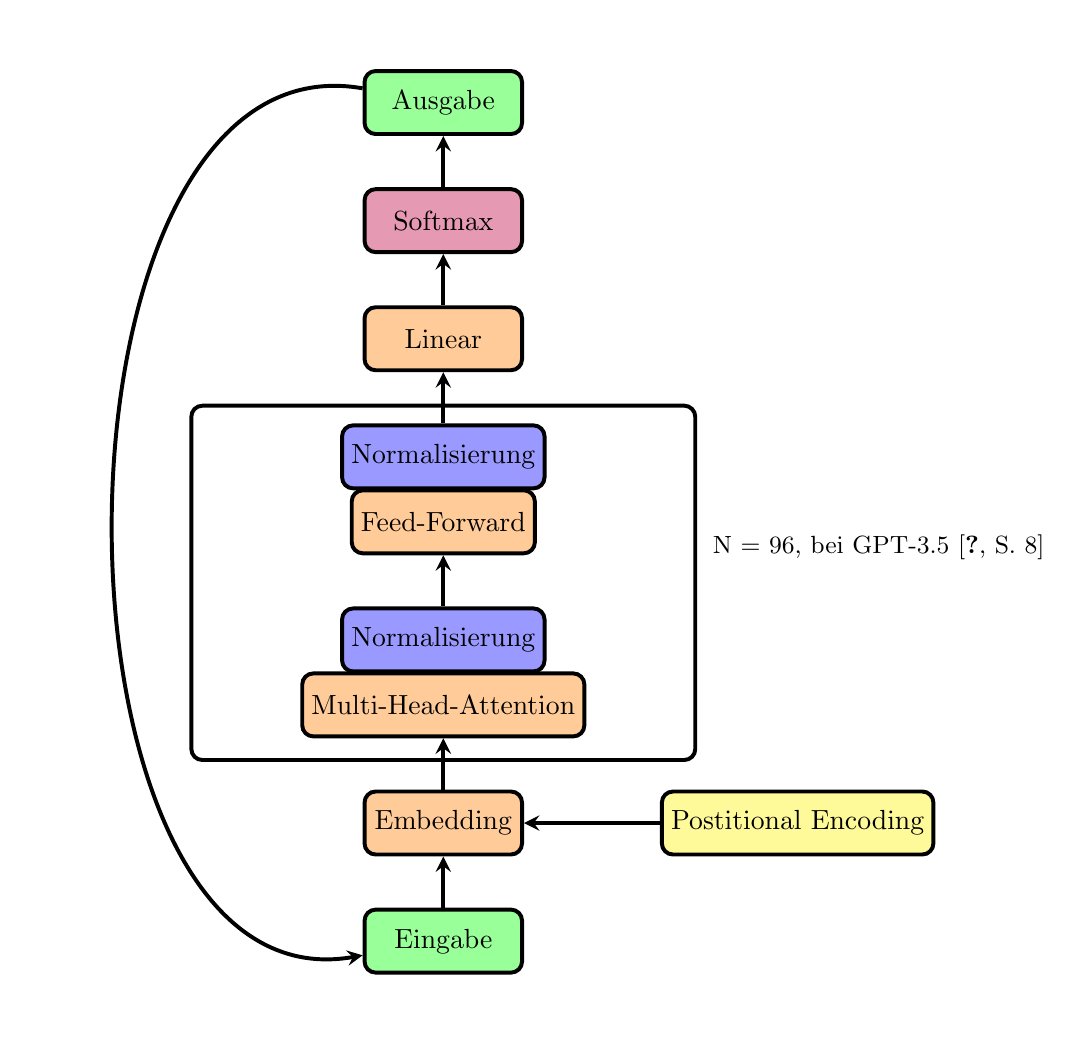
\begin{tikzpicture}[node distance=1.5cm]
		% Nodes
		\node (input) [concept, fill=green!40] {Eingabe};
		\node (embedding) [concept, above of=input] {Embedding};
		\node (encoding) [concept, right of=embedding, fill=yellow!40] (encoding) at (3, 1.5) {Postitional Encoding};
		\node (attention) [concept, above of=embedding] {Multi-Head-Attention};
		\node (normal) [concept, above of=attention, fill=blue!40] at (0, 2.325) {Normalisierung};
		\node (forward) [concept, above of=normal] {Feed-Forward};
		\node (normal1) [concept, above of=forward, fill=blue!40] at (0, 4.65) {Normalisierung};
		\node (linear) [concept, above of=normal1] {Linear}; 
		\node (softmax) [concept, above of=linear, fill=purple!40] {Softmax};
		\node (output) [concept, above of=softmax, fill=green!40] {Ausgabe};
		% Arrows
		\draw [arrow] (input) -- (embedding);	
		\draw [arrow] (encoding) -- (embedding);
		\draw [arrow] (embedding) -- (attention);
		\draw [arrow] (normal) -- (forward);
		\draw [arrow] (normal1) -- (linear);
		\draw [arrow] (linear) -- (softmax);
		\draw [arrow] (softmax) -- (output);
		\draw [arrow, bend right=100] (output) to (input);
		\draw[rounded corners, line width=0.5mm] (-3.2, 2.3) rectangle (3.2, 6.8);  
		\node[right] at (3.3, 5) {\small{N = 96, bei GPT-3.5 \cite[S. 8]{openAI2020}}};
		%\draw [highlight] (input) -- ++(-1,1) -- ++(4,0) -- ++(0,-2) -- cycle;
	\end{tikzpicture}
	
	\noindent
	Die Grafik veranschaulicht den Aufbau eines Transformers, welcher im Folgenden genauer erklärt wird. 
	
	Die erste Aufgabe eines Chatbots ist es Text in einzelne Tokens aufzuteilen und dann diesen Tokens 
	einen individuellen Vektor zuzuordnen. Das wird auch als Embedding bezeichnet. Durch das Umwandeln von Tokens in 
	einen Vektor kann das Netzwerk Text mathematisch verarbeiten. Weil die einzelnen Tokens nicht der Reihe, nach sondern 
	unabhängig voneinander und parallel zueinander verarbeitet werden, muss deren Position im Satz mit in den Eingabevektor des Tokens 
	encodiert werden \cite[S. 2f]{vaswani2017}. Das liegt daran, dass bei vielen Wörtern die Position im Satz eine 
	entscheidende Rolle dabei spielt, was der Satz aussagt:

	\vspace{3mm}
	\emph{Der Mann jagt den Hund.} 	
	\space $\neq$ \space
	\emph{Der Hund jagt den Mann.}
	
	\clearpage
	\noindent
	Nach dem Embedding folgt die Multi-Head Attention Schicht.
	Im Fall eines generativen Transformers wird sich hier der Self-Attention Mechanismus zunutze gemacht \cite[S. 2f]{turner2024}. 
	Dabei wird zunächst errechnet wie stark der Zusammenhang zwischen zwei Tokens ist \cite[S. 4]{vaswani2017}. Hat man zum 
	Beispiel die Frage, \emph{Wie nennt man ein großes Haus?} als Eingabe, könnten die errechneten Zusammenhänge für das 
	Wort Haus so aussehen: 
	
	\vspace{5mm}
	\begin{tabular}{ |c|c| }
  		\hline
	  	\multicolumn{2}{|c|}{Zusammenhang mit Haus: } \\
	  	\hline
	  	\emph{Wie} & 0,046 \\
	  	\hline
	  	\emph{nennt} & 0,08 \\
		\hline
	  	\emph{man} & 0,023 \\
	  	\hline
		\emph{ein} & 0,12 \\
	  	\hline
		\emph{großes} & 0,7 \\
	  	\hline
		\emph{Haus} & 0,031 \\
		\hline
		\emph{?} & 0,001 \\
		\hline
	\end{tabular}
	\vspace{5mm}
	
	\noindent Weil sich das Adjektiv \emph{großes} auf das Nomen \emph{Haus} bezieht, erkennt ein trainierter Transformer hier
	einen starken Zusammenhang. Durch diese errechneten Zusammenhänge zwischen den Tokens kann das Netzwerk abwägen, welches
	Token auf welches andere Token wie viel Einfluss nehmen soll.
		
	Auf die Multi-Head Attention folgt eine Normalisierung, welche dabei hilft die Vektoren zu verarbeiten. 
	Normalisierungen sind zwar Teil der Transformerachitektur aber nicht entscheidend für ein schematisches Verständnis
	und werden hier nicht beschrieben\cite[S.3]{vaswani2017}. 
	
	Der zweite bedeutende Teil eines Transformers nennt sich Feed-Forward-Block. Hier befinden sich c.a. 
	zwei Drittel der Parameter \cite{geva2024}. Parameter bestimmen bekannterweise die Ausgabewerte einer Funktion 
	also eines neuronalen Netzwerks. Im Fall eines Chatbots bestimmen diese Parameter, wie auf einen Satz, den der Transformer als 
	Eingabe bekommt, geantwortet wird. Bei diesen Antworten reicht es aber meistens nicht, einfach nur Zusammenhänge zwischen Wörtern 
	zu erkennen. Das LLM braucht Hintergrundwissen um einen großteil der Aufgaben zu bearbeiten, die ihm gestellt werden. 
	
	Im obigen Satz muss man zum Beispiel nicht nur verstehen, dass es um ein \emph{großes Haus} geht. Ebenfalls muss man wissen, dass alternative
	Wörter z. B. \emph{Wolkenkratzer} oder \emph{Plattenbau} lauten. Dafür braucht man den Feed-Forward-Block. Er kann als Gedächtnis des Transformers gesehen
	werden. Da sich hier ein Großteil der Parameter befindet, ist hier auch ein maßgeblicher Anteil des Wissens bzw. der Daten, die ein neuronales
	Netzwerk gelernt hat, gespeichert \cite{geva2024}.
	\vspace{5mm}
	
	Im Attention-Block werden also Zusammenhänge zwischen den Tokens erkannt und dann Informationen zwischen den Tokens übertragen
	und im Feed-Forward-Block wird dann den eingehenden Tokens bestimmtes Wissen, welches das Netzwerk besitzt, hinzugefügt.
	
	Wichtig ist, dass dieser Ablauf von Attention und Feed-Forward in einem Transformer mehrmals wiederholt wird, damit auch längere komplexe Texte mit
	komplizierten Zusammenhängen sinnvoll verarbeitet werden können.
	
	Am Ende des Transformers befinden sich noch eine lineare Schicht und eine Softmax Schicht. Diese sind dazu da die Ausgabe des Transformers
	in einen Vektor umzurechnen, der allen definierten Tokens eine Wahrscheinlichkeit zuweist \cite[S. 70]{nielsen2015}. Darunter wählt man 
	dann das wahrscheinlichste Token aus und fügt es dem Text hinzu. 	
	
	Die grundlegende Funktionsweise besteht also darin, dass der Transformer die Eingabe in Tokens (welche durch Vektoren repräsentiert wrden) 
	umwandelt, verarbeitet und dann als Ausgabe errechnet, welches Token mit welcher Wahrscheinlichkeit als Nächstes folgt. Natürlich wäre ein Chatbot der nur
	ein Token als Antwort geben könnte ziemlich nutzlos. Das Problem ist aber einfach zu lösen, indem man dem Transformer
	dieselbe Eingabe wie zuvor gibt aber noch dazu das neu generierte Token. Das wird auch als Selbstregression bezeichnet und 
	bedeutet, dass der Transformer seine Ausgabe wieder als Eingabe verwendet \cite[S. 2]{vaswani2017}. Diesen Prozess wiederholt 
	man so lange, bis der Transformer ein EOS-Token\footnote{End-of-Sequence-Token} generiert und damit den Abschluss seiner 
	Antwort signalisiert \cite[S. 2]{vaswani2017}.
	
	%chat gpt 3.5 tech report oder specs finden
	%aggarwal2018?
	\clearpage
	\subsection{Warum ist das noch nicht AGI?}\label{s2ss3}
	Bei AGI\footnote{Artificial General Intelligence} handelt es sich um eine Form der KI, die noch nicht existiert. 
	Bis jetzt verwenden wir ausschließlich ANI\footnote{Artificial Narrow Intelligence}, das ist KI die für 
	spizifische Aufgaben, wie z. B. Bilderkennung oder Textverarbeitung entwickelt wurde. In \ref{s1} wurde 
	herausgearbeitet, dass jedoch oft der Eindruck vermittelt wird, es handele sich bei modernen Chatbots um 
	eine Form von allgemeiner Intelligenz. Im Folgenden wird also herausgearbeitet, weshalb es sich bei den aktuellen Chatbots um ANI 
	handelt. Tatsächlich muss eine KI bestimmte Eigenschaften erfüllen, um als AGI bezeichnet werden zu können 
	\cite[S. 8]{goertzel23}:
	\begin{itemize}
	\item Eine AGI muss fähig sein ein breites Spektrum an Aufgaben unter verschiedenen Vorraussetzungen zu erledigen. 
	\item Eine AGI sollte auch mit Situationen oder Problemen umgehen können, für die sie nicht speziell entwickelt wurde. 
	\item AGI Systeme besitzen die Fähigkeit gelerntes Wissen von einem Problem auf ein anderes zu transferieren. 
	\end{itemize}	
	Zunächst einmal ist ein moderner Chatbot fähig verschiedenste Aufgaben zu erledigen. Man könnte auch argumentieren,
	dass durch die Bildverarbeitung und Tonverarbeitung, die diese Chatbots oft bereitstellen, verschiedene Vorraussetzungen 
	gelten, unter denen ein Chatbot seine Aufgaben erledigt. Die übrigen zwei Aspekte werden jedoch nicht erfüllt. 
	
	LLMs sind nicht oder nur begrenzt in der Lage mit Problemen umzugehen, die über das Verarbeiten von Text hinaus gehen. 
	Beispielsweise zeigt Ben Goertzel in seiner Arbeit, dass LLMs ein sehr begrenztes räumliches Vorstellungsvermögen haben 
	\cite[S. 32-35]{goertzel23}. Wenn Chatbots auf Fragen, die ein solches Vorstellungsvermögen verlangen, richtig antworten 
	wird meistens nur auf gelerntes Wissen zurückgegriffen, d.h. das LLM weiß die Antwort auswendig.
	
	Letztendlich fehlt modernen Chatbots vor allem die Fähigkeit erlerntes Wissen auf andere Probleme zu übertragen. Goertzel schreib in
	seiner Arbeit hierzu, dass ein Sprachmodell sein Wissen lediglich als Fallbeispiel abspeichert. Das führt dazu das dieses Wissen
	zwar je nach Bedarf abgerufen werden kann, aber nicht sinnvoll auf andere Situationen transferiert wird. LLMs fehlt eine 
	abstrakte Repräsentation des gelernten Wissens \cite[S. 81f]{goertzel23}. 
	
	\noindent{}Insgesamt ist man sich einig, dass es sich bei LLMs wie ChatGPT oder Gemini nicht um AGI handelt. Auch wenn nach außen
	hin oft der Eindruck vermittelt wird, man spräche mit einem allgemein intelligenten System, ist das nicht der Fall. 
	
	
\clearpage
\section{Was folgt daraus?}\label{s3}
	\subsection{Nur Algorithmen ohne Gefühle}\label{s3ss1}
	In \ref{s1ss1} wurde bereits gezeigt, dass KI-Chatbots teils mehr als nur nützliche Assistenten sein können.
	Jedoch muss die soziale Nutzung von Chatbots kritisch gesehen werden. Dafür gibt es folgende Gründe:

	Zunächst ist es wichtig zu verstehen, dass aktuelle Chatbots keine Gefühle empfinden, auch wenn es nach außen hin so wirkt.
	Wie bereits in \ref{s2ss2} gezeigt wurde handelt es sich bei modernen Chatbots um LLMs, also Programme, die durch Berechnung
	Texte generieren. Das LLM wird zunächst anhand von Beispieltext trainiert. Will man also, dass ein Chatbot fähig ist ein
	soziales Gespräch zu führen würde man ihn beispielsweise mit passenden Chatverläufen trainieren. Dadurch lernt der Chatbot
	zwar während sozialen Konversationen eine passende Antwort zu geben, jedoch versteht er dessen Bedeutung nicht \cite[S. 35-38]{goertzel23}.
	Das heißt also, dass Chatbots lediglich anhand von Trainingsdaten lernen so zu tun als hätten sie Gefühle. 

	Abgesehen von der Tatsache, dass Chatbots nicht in der Lage sind Gefühle zu empfinden, kann die vermehrte Nutzung von KI anstelle
	des Menschen zu einer Dehumanisierung führen. Indem man einem Chatbot menschliche Eigenschaften zuschreibt und Programme auf
	dasselbe Level wie reale Menschen stellt, verliert die soziale Interaktion mit echten Menschen an Bedeutung. Außerdem wird die
	soziale Komponente des Menschen dadurch ersetzbar gemacht, wodurch sie an Wert verliert \cite{chen24}. 	 

	Natürlich gibt es auch positive Aspekte, die eine Nutzung von KI in sozialen Bereichen mit sich bringt. Die aufgeführten Gründe
	zeigen aber, dass man zwischen der Verwendung von AEI und Interaktionen mit realen Menschen differenzieren sollte.
	  
	%1. KI ist nicht wirklich intellegent, wurde darauf trainiert so zu tun als hätte sie emotionen!!! JA!
	%1. KI hat eigentlich keine emotionen JA!
	%Other. negative einflüssen, wenn man zu sozial abhängig von KI wird
	\clearpage
	\subsection{Falsche Darstellung in den Medien}\label{s3ss2}
	Die genannten Beispiele aus \ref{s1ss3} sollen im folgenden Teil erneut aufgegriffen und richtig gestellt werden. Darüber
	hinaus werden die technischen Hintergründe zu den Beispielen genauer beleuchtet. 

	Zu Beginn wurde auf die Gemini Demo eingegangen. Im Video zur Demo wurde vor allem betont, wie Interaktiv der Chatbot mit
	der anwesenden Person zusammenarbeitet und es entsteht der Eindruck, dass der Chatbot in Echtzeit auf die Person reagiert.
	In Wahrheit hat der Chatbot aber nur Bilder und Text mit zusätzlichen Hinweisen als Eingabe bekommen \cite{chenGoogle23}. Beispielsweise wurde
	dem Chatbot das folgende Bild gezeigt, mit dem Hinweis, dass es sich um ein Spiel handelt:
	\begin{figure}[h]
    	
\includegraphics[scale=0.25]{assets/hand_rock_paper_scissors.png}
    \end{figure}
	\newline
	Der Chatbot hat also nicht durch eine Echtzeitaufnahme anhand von Handbewegungen erkannt, dass es sich um das Spiel \glqq{}Schere
	Stein Papier\grqq{} handelt, sondern durch ein Bild mit zusätzlichem Hinweis. Dieses Schema zieht sich durch das gesamte Video und
	es wird nicht erwähnt, dass der Chatbot ausschließlich Bilder mit zusätzlichem Text als Eingabe erhält. Obwohl in der Beschreibung des
	Videos ein Artikel verlinkt ist, indem die Erstellung verdeutlicht wird, hat das Video bei vielen Leuten für falsche
	Erwartungen und letztendlich für Kritik gesorgt.

	Das zweite Beispiel bezog sich auf einen Artikel, indem die Funktionsweise und das Training von Chatbots erklärt wird. Im 
	Artikel wird mehrmals erwähnt, dass Chatbots aus den Konversationen mit den Nutzern lernen \cite{gramsch23}. In \ref{s2ss2} wurde genauer 
	erklärt, wie ein Chatbot auf Nutzeranfragen antwortet. Während der Chatbot eine Antwort generiert findet kein Training statt, da die Parameter
	des Transformers nicht verändert werden. Die Aussage, dass der Chatbot aus den Fragen der Nutzer lernt ist also falsch.	

	\clearpage
	\noindent
	Beide genannten Fälle sorgen dafür, dass KI besser dargestellt wird, als sie eigentlich
	ist. Dafür gibt es mehrere Hintergründe, wie z. B. Marketing im Fall von Gemini oder mangelndes
	Wissen. Problematisch ist, dass vor allem Personen, die nur wenig Verständnis von KI besitzen, durch 
	solche Informationsquellen leicht einen falschen Eindruck davon bekommen können, wozu Chatbots fähig sind.
	
	\clearpage
	\subsection{IQ-Tests mit wenig Aussagekraft}\label{s3ss3}
	Kapitel \ref{s1ss3} hat IQ-Tests im Zusammenhang mit Chatbots behandelt. Dabei wurde erklärt, wie ChatGPT-4 in einem
	IQ-Test eine Punktezahl von 155 erzielte. Im Folgenden soll diskutiert werden, warum dieses Ergebnis nicht mit dem
	eines Menschen vergleichbar ist und kritisch gesehen werden muss.
	
	Zum einen wurde nur ein verbaler IQ-Test durchgeführt. Natürlich hat man bei einem textbasierten Chatbot 
	keine andere Möglichkeit Fragen zu stellen. Roivainen schreibt in seinem Artikel, dass der verbale und allgemeine IQ
	stark zusammenhängen. Er erklärt, dass ChatGPT nach menschlichen Maßstäben sehr intelligent ist \cite{roivainen23}.
	Der Zusammenhang zwischen verbalen und allgemeinen IQ wurde jedoch bei Menschen und nicht bei Chatbots beobachtet. Darum
	ist diese Folgerung so nicht möglich.
	
	Zudem sind die Fragen, die der Chatbot beantwortet hat, nicht geeignet, wenn es darum geht festzustellen, wie intelligent eine KI ist.
	Bekommt ein Mensch z. B. die Frage \glqq{}Was haben Harry Potter und Bugs Bunny gemeinsam\grqq{} \cite{roivainen23},
	dann muss er nachdenken, wodurch man einen sinnvollen Zusammenhang zwischen Bugs Bunny und Harry Potter herstellt.
	Bekommt hingegen ein Chatbot diese Frage, dann kann er sie meistens anhand der Trainingsdaten beantworten. Ein Chatbot
	kommt nicht auf dieselbe Weise zu einer Antwort wie ein Mensch. Das wird in \ref{s2ss2} deutlich. Daraus folgt auch,
	dass man die Ergebnisse von Menschen und Chatbots in solchen IQ-Test nicht sinnvoll vergleichen kann. Somit ist die
	Folgerung von Roivainen, dass ChatGPT nach menschlichen Maßstäben sehr intelligent ist, nicht zutreffend \cite{roivainen23}. 
	Außerdem wurde in \ref{s2ss3} gezeigt, dass es sich bei Chatbots nicht um allgeimeine Intelligenz handelt. Ihnen fehlen essenzielle
	Eigenschaften, die eine zentrale Rolle bei der Definition von allgemeiner Intelligenz spielen. 	
	
	Das Ergebnis, welches ChatGPT-4 im WAIS-III IQ-Test erzielt hat, wurde mehrmals zitiert. Wie im Artikel selbst wurde die
	Vergleichbarkeit zwischen Mensch und Chatbot einfach vorausgesetzt \cite{gawdat23} oder nicht kritisch hinterfragt 
	\cite{blutermann23}. Durch das aufgeführte Beispiel wird deutlich, wie leicht Ergebnisse, die KI in IQ-Tests erzielt, missverstanden
	werden können. Allgemein ist es sehr schwer die Intelligenz eines Chatbots mit der eines Menschen zu vergleichen. 
	%goeartzel ???
	
\clearpage
\section{Fazit: KI kann missverstanden werden}
Zusammenfassend lässt sich feststellen, dass es durchaus möglich ist, eine falsche Auffassung von KI zu bekommen. Dazu braucht es nicht
einmal direkt falsche Informationen, sondern vor allem eine mangelnde Intuition, was tatsächlich hinter den aktuellen Chatbots steckt.
Es ist wichtig grundlegend zu verstehen wie Chatbots funktionieren, um Neuigkeiten und Informationen über Chatbots richtig einordnen zu können.   
Das wurde in der Arbeit durch folgende drei Beispiele verdeutlicht.

Chatbots stellen für einige Menschen einen sozialen Mehrwert dar. Personen, die Chatbots für diese Zwecke verwenden sollten sich bewusst sein,
dass Chatbots keine Empfindungsfähigkeit besitzen. Zudem sollte man klar zwischen der sozialen Interaktion mit Chatbots und der mit Menschen unterscheiden.

Die Medien spielen eine zentrale Rolle dabei, die Öffentlichkeit über Neuigkeiten zum Thema KI und Chatbots zu informieren. Das heißt jedoch nicht,
dass Informationen, die in den Medien vermittelt werden, richtig sind. Mit einem grundlegenden Verständnis ist es aber deutlich leichter zwischen richtigen und
falschen Informationen zu unterscheiden.     

Auch wenn ein Chatbot nach außen hin sehr intelligent wirkt und man das auch mit einem IQ-Test messen kann, muss man die Ergebnisse von Chatbots
und Menschen unterscheiden. Chatbots haben zahlreiche Schwächen und Einschränkungen, die sich aber nicht direkt bemerkbar machen. 

Natürlich konnte im Rahmen dieser Arbeit nur ein Teil der Faktoren, die die öffentliche Wahrnehmung von Chatbots beeinflussen, behandelt werden. 
Es gibt auch zahlreiche gute Quellen, um sich über KI zu informieren. Die Arbeit hat aber deutlich gemacht, dass man leicht auf falsche Informationen
stoßen kann.

Letztendlich werden Chatbots bzw. KI immer mehr in unser modernes Leben integriert. Aus diesem Grund wird auch ein Verständnis dieser Technologie immer wichtiger
um damit verantwortungsvoll umgehen zu können und Missverständnisse zu vermeiden. Darum bietet diese Arbeit eine vereinfachte Erklärung von GPTs, 
die den Leserinnen und Lesern einen Einblick in das Thema Künstliche Intelligenz gibt und ihnen dabei hilft, die Funktionsweise und die Grenzen dieser 
Technologie besser zu verstehen. 


%welches bild hat die öffentlichkeit also bzw. wie denkt sie über ki?
